% 第6章第8节：矩阵的长期作用（谱半径判据、衰减速度与边界情形、瞬态放大、Neumann级数）。

\section{矩阵的长期作用}
\label{sec:ls-convergence}
\label{sec:linear-algebra-convergence-approximation}
\label{sec:ls-matrix-power-behavior}
\label{sec:linear-algebra-power-convergence}

条件数衡量的是一次作用的放大。迭代法、离散动态系统和许多学习算法却反复施加同一个线性作用，得到序列$\bm x^{(k)}=\bm A^k\bm x^{(0)}$；把这些作用累加起来，又得到矩阵级数。本节回答两个问题。第一，矩阵幂什么时候对所有初值都趋于零，趋近得多快，途中会不会先变大？第二，由矩阵幂组成的级数什么时候收敛，收敛到什么？

讨论收敛时不必担心范数的选择。第~\ref{sec:ls-finite-dimensional-sequences}节已经说明，有限维空间上的任意两个范数彼此等价（定理~\ref{thm:ls-norm-equivalence}），向量或矩阵序列是否收敛与所用范数无关，换范数只改变不等式中的常数。所以下面可以在任意方便的范数下论证，结论对所有范数成立。我们将看到，长期行为由谱半径决定，早期的放大则取决于矩阵是否正规。

\subsection{谱半径判据}

对固定方阵$\bm A$反复作用，初值$\bm x^{(0)}$在第$k$步变成$\bm x^{(k)}=\bm A^k\bm x^{(0)}$。只检查一个初值的轨迹不够：若初值恰好不含某个增长方向的分量，轨迹看起来收敛，换一个初值就发散。下面的反例说明这一点。
\begin{example}[反例：收敛与发散的轨迹]
\label{ex:ls-partial-convergence}
给定$\bm A=\operatorname{diag}(0.5,2)$，比较两个初值的轨迹：
\[
 \bm A^k\begin{bmatrix}1\\0\end{bmatrix}=\begin{bmatrix}0.5^k\\0\end{bmatrix}\to\bm0,\qquad
 \bm A^k\begin{bmatrix}0\\1\end{bmatrix}=\begin{bmatrix}0\\2^k\end{bmatrix},
\]
其中后一条轨迹的长度为$2^k\to\infty$。
结论：初值$(1,0)^\top$不含增长方向$\bm e_2$的分量，轨迹收敛；初值$(0,1)^\top$的轨迹发散。一个初值的轨迹收敛，不能说明矩阵幂趋于零。
\end{example}
所以要问的是：何时对全体初值都有$\bm A^k\bm x^{(0)}\to\bm0$？逐个取$\bm x^{(0)}=\bm e_j$可知，这等价于$\bm A^k$的每一列趋于零，即$\bm A^k\to\bm0$。

图~\ref{fig:ls-spectral-radius-convergence}显示了最简单的正规情形：误差每步乘以$\rho$，$\rho<1$时衰减，$\rho>1$时增长。

\begin{figure*}[htbp]
 \centering
 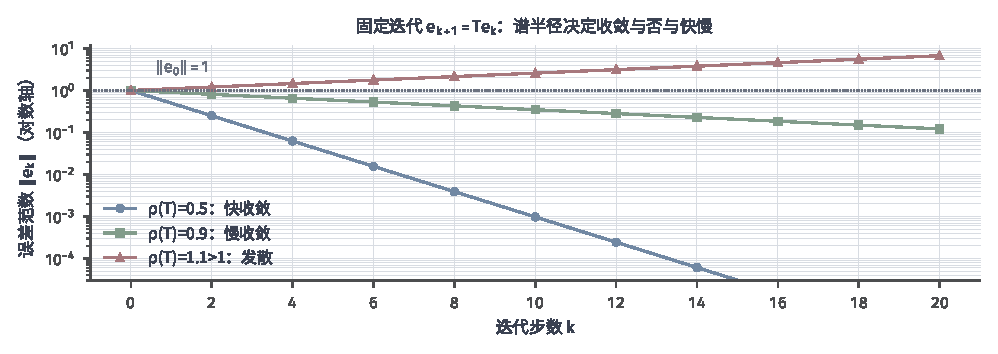
\includegraphics[width=169.0mm]{figures/01-mathematical-preliminaries-upper/02-linear-spaces/matplotlib/ls-spectral-radius-convergence/ls-spectral-radius-convergence.pdf}
 \caption{谱半径决定迭代的长期方向。递推$\bm e^{(t+1)}=\bm A\bm e^{(t)}$、
 $\lVert\bm e^{(0)}\rVert=1$，取正规矩阵$\bm A=\rho\bm I$时$\lVert\bm e^{(t)}\rVert=\rho^t$：
 $\rho=0.5$（蓝）约十四步降到$10^{-4}$，$\rho=0.9$（绿）缓慢下降，
 $\rho=1.1$（红）指数上升。纵轴为半对数。}
 \label{fig:ls-spectral-radius-convergence}
\end{figure*}

最先想到的判据来自范数。由次乘性，$\lVert\bm A^k\rVert\leq\lVert\bm A\rVert^k$，所以只要在某个次乘性矩阵范数下$\lVert\bm A\rVert<1$，就有$\bm A^k\to\bm0$。但这只是充分条件：示例~\ref{ex:ls-nonnormal-norm-radius}的矩阵$\left[\begin{smallmatrix}0.8&4\\0&0.5\end{smallmatrix}\right]$二范数大于$4$，而示例~\ref{ex:ls-triangular-power}已经算出它的幂按$0.8^k$与$0.5^k$趋于零，它的谱半径也只有$0.8$。正规矩阵的范数等于谱半径；非正规矩阵的Schur形中，非对角块以及不呈模长乘旋转形式的$2\times2$对角块都会使范数大于谱半径。下面的引理先用相似变换把每个对角块化为模长乘旋转，再用一次坐标缩放把非对角块压小，从而把谱半径变成一个可用的几何上界。

\begin{lemma}[矩阵幂的几何上界]
\label{lem:ls-power-geometric-bound}
对任意$r>\rho(\bm A)$，存在常数$C_r$，使$\lVert\bm A^k\rVert_2\leq C_rr^k$对所有$k\geq0$成立；等价地，存在一个向量范数，使$\bm A$在它诱导的矩阵范数下不超过$r$。
\end{lemma}
\begin{proof}
取实Schur形$\bm A=\bm Q\bm T\bm Q^\top$，设$\bm T$有$s$个对角块，第$i$块的特征值模长为$|\lambda_i|$。

先处理对角块。每个$2\times2$对角块$\bm T_{i,i}$有一对共轭特征值，按第~\ref{sec:ls-general-square-spectrum}节的论证，在复特征向量的实部、虚部组成的基下，它化为模长乘旋转：$\bm T_{i,i}=\bm P_i(|\lambda_i|\bm R_i)\bm P_i^{-1}$，$\bm R_i$为旋转矩阵；$1\times1$块取$\bm P_i=1$、$\bm R_i=\pm1$。

再压小非对角块。对$0<\varepsilon\leq1$，令分块对角矩阵
\[
 \bm D_\varepsilon=\operatorname{diag}(\varepsilon^{0}\bm P_1,\varepsilon^{1}\bm P_2,\ldots,\varepsilon^{s-1}\bm P_s).
\]
直接相乘，$\bm D_\varepsilon^{-1}\bm T\bm D_\varepsilon$的第$(i,j)$块为$\varepsilon^{j-i}\bm P_i^{-1}\bm T_{i,j}\bm P_j$：对角块是$|\lambda_i|\bm R_i$，二范数不超过$\rho(\bm A)$；$j>i$的块带有因子$\varepsilon^{j-i}\leq\varepsilon$，所以全部非对角块的Frobenius范数不超过$\varepsilon c$，其中$c$与$\varepsilon$无关。把矩阵拆成分块对角部分与非对角部分，得
\[
 \lVert\bm D_\varepsilon^{-1}\bm T\bm D_\varepsilon\rVert_2\leq\rho(\bm A)+\varepsilon c .
\]
取$\varepsilon$足够小，使右端不超过$r$。

最后换回原坐标。令$\bm M=\bm Q\bm D_\varepsilon$，则$\bm A=\bm M(\bm D_\varepsilon^{-1}\bm T\bm D_\varepsilon)\bm M^{-1}$，中间各对$\bm M^{-1}\bm M$相消，$\bm A^k=\bm M(\bm D_\varepsilon^{-1}\bm T\bm D_\varepsilon)^k\bm M^{-1}$，故
\[
 \lVert\bm A^k\rVert_2\leq\lVert\bm M\rVert_2\lVert\bm M^{-1}\rVert_2\,r^k ,
\]
取$C_r=\lVert\bm M\rVert_2\lVert\bm M^{-1}\rVert_2$即可。所求的向量范数取$\bm x\mapsto\lVert\bm M^{-1}\bm x\rVert_2$，它诱导的$\bm A$的范数等于$\lVert\bm M^{-1}\bm A\bm M\rVert_2=\lVert\bm D_\varepsilon^{-1}\bm T\bm D_\varepsilon\rVert_2\leq r$。
\end{proof}

有了这个上界，就能给出矩阵幂衰减的充要条件。
\begin{theorem}[矩阵幂的衰减判据]
\label{thm:ls-power-decay}
对实方阵$\bm A$，$\bm A^k\to\bm0$当且仅当$\rho(\bm A)<1$。
\end{theorem}
\begin{proof}
充分性：取$r$满足$\rho(\bm A)<r<1$，由引理，$\lVert\bm A^k\rVert_2\leq C_rr^k\to0$。必要性：设有特征值$|\lambda|\geq1$。若$\lambda$为实数，其特征向量$\bm v$满足$\lVert\bm A^k\bm v\rVert=|\lambda|^k\lVert\bm v\rVert\not\to0$；若$\lambda$非实，在对应的二维不变子空间中，$\bm A^k$在基$(\bm u,\bm w)$下的矩阵是$|\lambda|^k$乘一个旋转，$\bm A^k\bm u$的坐标长度为$|\lambda|^k\geq1$，不趋于零。两种情形都有$\bm A^k\not\to\bm0$。
\end{proof}

\subsection{衰减速度与边界情形}

判据只回答矩阵幂是否趋于零，同一论证还给出衰减速度。上界$\lVert\bm A^k\rVert\leq C_rr^k$对任意$r>\rho(\bm A)$成立；必要性证明中的特征方向（或不变平面）给出下界$\lVert\bm A^k\rVert\geq c\,\rho(\bm A)^k$，$c>0$为常数。两边开$k$次方，$C_r^{1/k}$与$c^{1/k}$都趋于$1$，于是$\rho(\bm A)\leq\liminf_k\lVert\bm A^k\rVert^{1/k}\leq\limsup_k\lVert\bm A^k\rVert^{1/k}\leq r$。令$r$趋于$\rho(\bm A)$，得到Gelfand公式
\begin{equation}
 \rho(\bm A)=\lim_{k\to\infty}\lVert\bm A^k\rVert^{1/k}.
 \label{eq:ls-gelfand-formula}
\end{equation}
由范数等价（定理~\ref{thm:ls-norm-equivalence}），换成任意矩阵范数只改变常数，开$k$次方后常数的影响消失，所以公式对任意矩阵范数成立。由$\lVert\bm A^k\rVert\leq\lVert\bm A\rVert^k$还得$\rho(\bm A)\leq\lVert\bm A\rVert$对任意次乘性范数成立。

Gelfand公式说明，谱半径是每步放大倍数的长期几何平均：长期看，误差每步大约乘以$\rho(\bm A)$。由$\rho^m=1/10$解出，把误差缩小$10$倍约需$m=1/\log_{10}(1/\rho)$步，$\rho=0.5$时约$3.3$步，$\rho=0.99$时约$229$步；$\rho$越接近$1$，收敛越慢。

$\rho(\bm A)=1$是边界情形，结果取决于模为$1$的特征值。特征值$1$的特征方向保持不动，$-1$的特征方向来回翻转，模为$1$的非实特征值对应纯旋转；在这些方向上$\bm A^k$不趋于零，但保持有界。若模为$1$的特征值缺少足够的特征向量，还会出现增长。
\begin{example}[反例：谱半径为$1$而矩阵幂无界]
\label{ex:ls-unit-spectral-radius-growth}
给定$\bm J_1=\left[\begin{smallmatrix}1&1\\0&1\end{smallmatrix}\right]$，它只有特征值$1$，$\rho(\bm J_1)=1$，特征向量只有$(1,0)^\top$的倍数。按示例~\ref{ex:ls-jordan-block-power}的二项式展开，把$0.8$换成$1$，得
\[
 \bm J_1^k=(\bm I+\bm N)^k=\bm I+k\bm N=\begin{bmatrix}1&k\\0&1\end{bmatrix}.
\]
结论：右上角随$k$线性增长，$\lVert\bm J_1^k\rVert_2\geq k\to\infty$；谱半径等于$1$不能保证矩阵幂有界。
\end{example}
$\rho(\bm A)>1$时，由定理~\ref{thm:ls-power-decay}必要性的证明，从模大于$1$的特征值的特征方向（或不变平面）出发的轨迹不趋于零；但如示例~\ref{ex:ls-partial-convergence}所示，不必每个初值都发散。

\subsection{非正规矩阵的瞬态放大}

$\rho(\bm A)<1$保证最终衰减，但不说明途中的情况。下面的例子中，轨迹先变长、后衰减。
\begin{example}[非正规矩阵的瞬态放大]
\label{ex:ls-transient-growth}
给定迭代
\begin{equation}
 \bm A=\begin{bmatrix}0.8&4\\0&0.5\end{bmatrix},\qquad
 \bm x^{(k+1)}=\bm A\bm x^{(k)},\qquad \bm x^{(0)}=(0,1)^{\top}.
 \label{eq:ch06-fixed-iteration-example}
\end{equation}
示例~\ref{ex:ls-triangular-power}已把初值沿特征向量$\bm v_1=(1,0)^{\top}$、$\bm v_2=(-40/3,1)^{\top}$分解为$\bm x^{(0)}=\tfrac{40}{3}\bm v_1+\bm v_2$，并写出了矩阵幂与轨迹：
\begin{equation}
 \bm A^k=
 \begin{bmatrix}
  0.8^k&\frac{40}{3}(0.8^k-0.5^k)\\
  0&0.5^k
 \end{bmatrix},\qquad
 \bm x^{(k)}=
 \begin{bmatrix}\frac{40}{3}(0.8^k-0.5^k)\\0.5^k\end{bmatrix}.
 \label{eq:ch06-diagonalizable-finite-trajectory}
\end{equation}
代入$k=1,2,3$得
\[
 \bm x^{(1)}=\begin{bmatrix}4\\0.5\end{bmatrix},\qquad
 \bm x^{(2)}=\begin{bmatrix}5.2\\0.25\end{bmatrix},\qquad
 \bm x^{(3)}=\begin{bmatrix}5.16\\0.125\end{bmatrix},
\]
长度分别约为$4.03$、$5.21$、$5.16$，都远大于初值的长度$1$。另一方面$\rho(\bm A)=0.8<1$，由定理~\ref{thm:ls-power-decay}，轨迹最终趋于零。结论：谱半径小于$1$时，轨迹仍可以先放大数倍、再衰减。
\end{example}
放大的原因在于初值的分解。$\tfrac{40}{3}\bm v_1=(40/3,0)^\top$与$\bm v_2=(-40/3,1)^\top$都很长、方向几乎相反，初值$(0,1)^\top$由二者相消而成。两个分量衰减速度不同，相消很快被打破，所以长度先增后降（图~\ref{fig:ch06-transient-growth}）。

\begin{figure*}[htbp]
  \centering
  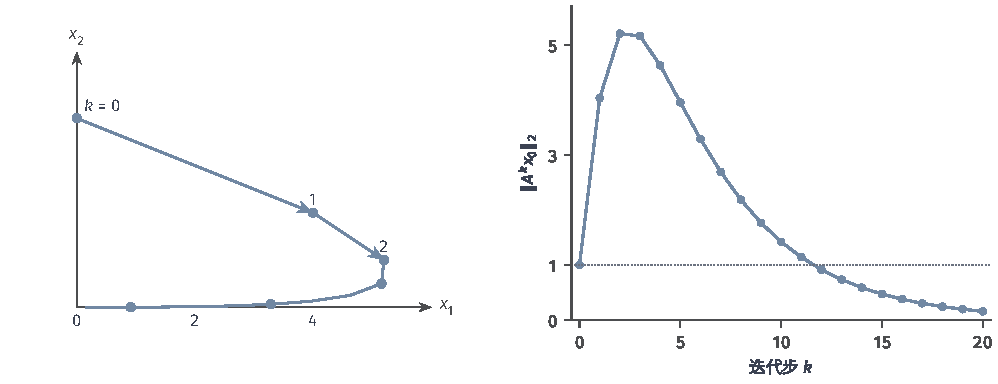
\includegraphics[width=169.0mm]{figures/01-mathematical-preliminaries-upper/02-linear-spaces/matplotlib/ch06-transient-growth/figure.pdf}
  \caption{固定二维矩阵的反复作用。初值为$(0,1)^{\top}$，前两步的长度增加，
  此后回到原点；右图将长度与初始长度$1$比较。特征值$0.8$和$0.5$决定长期衰减，
  非正交特征方向间的相消则决定早期放大。两图使用同一个矩阵和同一组迭代点。}
  \label{fig:ch06-transient-growth}
\end{figure*}

一般地，可对角化矩阵$\bm A=\bm V\bm\Lambda\bm V^{-1}$满足$\bm A^k=\bm V\bm\Lambda^k\bm V^{-1}$，所以
\[
 \lVert\bm A^k\rVert_2\leq\lVert\bm V\rVert_2\lVert\bm V^{-1}\rVert_2\,\rho(\bm A)^k .
\]
特征向量越接近线性相关，$\lVert\bm V\rVert_2\lVert\bm V^{-1}\rVert_2$越大，早期可能的放大越强。正规矩阵则满足$\lVert\bm A^k\rVert_2=\rho(\bm A)^k$（第~\ref{sec:ls-general-square-spectrum}节），不会出现瞬态放大。

不可对角化时，特征向量本身就不够，矩阵幂中还会出现多项式因子。考虑$s$阶矩阵$\bm J=\lambda\bm I+\bm N$，其中$\bm N$是超对角元为$1$、其余元素为零的矩阵，满足$\bm N^s=\bm0$；这样的矩阵称为Jordan块，示例~\ref{ex:ls-jordan-block-power}的$\bm J$是$s=2$的情形。$\lambda\bm I$与$\bm N$可交换，二项式展开成立，且$j\geq s$的项为零：
\begin{equation}
 \bm J^k=\sum_{j=0}^{\min(k,s-1)}\binom{k}{j}\lambda^{k-j}\bm N^j .
 \label{eq:ch06-jordan-power}
\end{equation}
$\binom kj$是$k$的至多$s-1$次多项式，而多项式增长慢于几何衰减，$k^{s-1}|\lambda|^k\to0$（$|\lambda|<1$）。所以$|\lambda|<1$时块幂仍趋于零，只是起初可能上升。下面用二阶块看这种先升后降。
\begin{example}[Jordan块幂的先升后降]
\label{ex:ls-jordan-transient}
给定$\bm J=\left[\begin{smallmatrix}0.8&1\\0&0.8\end{smallmatrix}\right]$与初值$(0,1)^{\top}$。由示例~\ref{ex:ls-jordan-block-power}，
\[
 \bm J^k\begin{bmatrix}0\\1\end{bmatrix}=\begin{bmatrix}k\,0.8^{k-1}\\0.8^k\end{bmatrix}.
\]
第一坐标在$k=1,2,\ldots,6$时依次为$1$、$1.6$、$1.92$、$2.048$、$2.048$、$1.966$（末项保留三位小数），在$k=4,5$时达到最大值约$2.05$，此后才衰减。结论：特征值$0.8<1$保证最终衰减，但多项式因子$k$使第一坐标先上升到初值长度的两倍以上。
\end{example}
图~\ref{fig:vol1-add-linear-jordan-accumulation}画出这条轨迹的两个坐标。多项式因子也是引理~\ref{lem:ls-power-geometric-bound}中常数$C_r$的来源：$r$越接近$\rho(\bm A)$，需要的$\varepsilon$越小，$C_r$可能越大。

\begin{figure}[!htb]
  \centering
  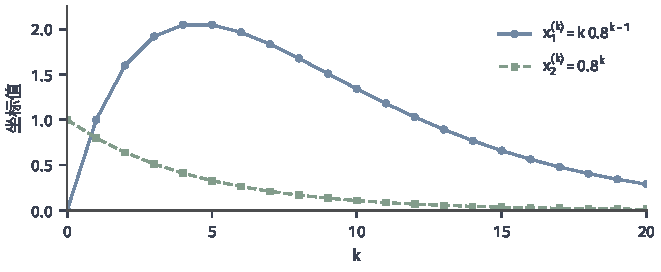
\includegraphics[width=112mm]{figures/01-mathematical-preliminaries-upper/02-linear-spaces/matplotlib/comprehension-additions/linear-jordan-accumulation.pdf}
  \caption{Jordan块的累积项。取正文$\bm J=\left[\begin{smallmatrix}0.8&1\\0&0.8\end{smallmatrix}\right]$与初值$(0,1)^{\top}$。绿线为$0.8^k$，蓝线在$k\geq1$时为$k0.8^{k-1}$，在$k=0$时为$0$。点表示整数步，连线仅引导读图；两坐标最终都趋零。}
  \label{fig:vol1-add-linear-jordan-accumulation}
\end{figure}

所以报告迭代的收敛性时，要分开两件事：谱半径给出长期速度，特征向量的病态程度或Jordan块决定早期可能的放大。

\subsection{Neumann级数}
\label{sec:ls-matrix-series-exponential}

把矩阵幂累加起来会得到什么？最常用的是$\sum_k\bm A^k$，它把求逆$(\bm I-\bm A)^{-1}$写成反复作用之和，也描述每步注入的误差怎样累积。这里说矩阵级数$\sum_{k=0}^{\infty}\bm A^k$收敛，指部分和$\bm S_N=\sum_{k=0}^N\bm A^k$作为矩阵序列收敛。对标量$a$，$|a|<1$时几何级数$\sum_ka^k=1/(1-a)$；矩阵情形有同样的结论。

\begin{theorem}[Neumann级数与逆]
\label{thm:ls-neumann}
若在某个次乘性矩阵范数下$\lVert\bm A\rVert<1$，则级数$\sum_{k=0}^{\infty}\bm A^k$收敛，$\bm I-\bm A$可逆，且
\begin{equation}
 (\bm I-\bm A)^{-1}=\sum_{k=0}^{\infty}\bm A^k,
 \label{eq:ls-neumann-series}
\end{equation}
截断尾项满足$\lVert\sum_{k>N}\bm A^k\rVert\leq\lVert\bm A\rVert^{N+1}/(1-\lVert\bm A\rVert)$。
\end{theorem}
\begin{proof}
由次乘性，$\sum_k\lVert\bm A^k\rVert\leq\sum_k\lVert\bm A\rVert^k<\infty$。由范数等价（定理~\ref{thm:ls-norm-equivalence}），每个元素的绝对值不超过常数乘$\lVert\bm A^k\rVert$，所以每个元素的级数绝对收敛，矩阵级数收敛到某个$\bm S$；尾界由几何级数求和得到。逐项相消，$(\bm I-\bm A)\bm S_N=\bm S_N(\bm I-\bm A)=\bm I-\bm A^{N+1}$，令$N\to\infty$，$\bm A^{N+1}\to\bm0$，得$(\bm I-\bm A)\bm S=\bm S(\bm I-\bm A)=\bm I$。
\end{proof}
条件$\lVert\bm A\rVert<1$可以放宽到谱半径。由引理~\ref{lem:ls-power-geometric-bound}，只要$\rho(\bm A)<1$，就存在使$\lVert\bm A\rVert<1$的诱导范数，所以级数在$\rho(\bm A)<1$时收敛，只是尾界要在那个范数中读取；反之$\rho(\bm A)\geq1$时，由定理~\ref{thm:ls-power-decay}，通项$\bm A^k$不趋于零，级数发散。图~\ref{fig:ls-neumann-series-tail}用一个$2\times2$例子核对尾界。

\begin{figure}[htbp]
 \centering
 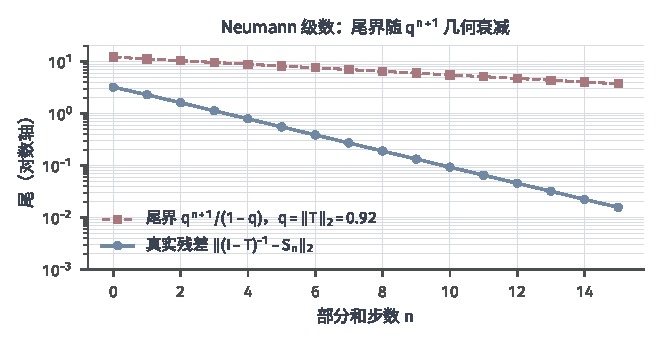
\includegraphics[width=112mm]{figures/01-mathematical-preliminaries-upper/02-linear-spaces/matplotlib/ls-neumann-series-tail/ls-neumann-series-tail.pdf}
 \caption{Neumann级数尾界。$\bm T=[[0.7,0.6],[0,0.1]]$，$q=\lVert\bm T\rVert_2
 \approx0.924<1$，$(\bm I-\bm T)^{-1}=\sum\bm T^k$。蓝线为真实残差
 $\lVert\bm R_n\rVert=\lVert\bm T^{n+1}(\bm I-\bm T)^{-1}\rVert$，红虚线为尾界
 $q^{n+1}/(1-q)$，纵轴半对数（$n=0,\dots,15$）。}
 \label{fig:ls-neumann-series-tail}
\end{figure}

\paragraph{持续扰动的累积}

同样的级数描述持续扰动的累积。迭代的每一步都可能引入新误差（例如舍入），递推成为$\bm e^{(t+1)}=\bm T\bm e^{(t)}+\bm\delta^{(t)}$，$\bm\delta^{(t)}$是第$t$步注入的误差。逐步展开，
\[
 \bm e^{(t)}=\bm T^t\bm e^{(0)}+\sum_{j=0}^{t-1}\bm T^{t-1-j}\bm\delta^{(j)} .
\]
若在某个范数下$\lVert\bm T\rVert\leq q<1$且$\lVert\bm\delta^{(j)}\rVert\leq\delta$，第二项不超过$\delta\sum_{i\geq0}q^i$，于是
\begin{equation}
 \lVert\bm e^{(t)}\rVert\leq q^t\lVert\bm e^{(0)}\rVert+\frac{\delta}{1-q}.
 \label{eq:ls-noise-floor}
\end{equation}
初始误差几何衰减，持续扰动却留下不随$t$下降的误差下限$\delta/(1-q)$；$q$越接近$1$，下限越高。

本节的两个问题至此都有了回答。矩阵幂对全体初值衰减，当且仅当谱半径小于$1$；谱半径还是每步放大倍数的长期几何平均，决定收敛快慢。非正规矩阵在衰减之前可能先放大，放大程度由特征向量的病态程度或不可对角化的结构决定。Neumann级数在谱半径小于$1$时收敛到$(\bm I-\bm A)^{-1}$，持续注入的扰动则留下不随步数下降的误差下限。
